\subsubsection{Rendu avec OpenGL}
L'ensemble des rendus est réalisé avec OpenGL et des shaders écrits en GLSL. Lorsque un objet est chargé dans la scène, le chargeur d'objet remplit des tableaux tels que la position des sommets, les couleurs et les normales associées aux sommets, et les indices associés aux sommets de chaque faces.\\
Certains fichiers d'objet posent problème, notamment les fichiers avec le format .ply, qui ne possèdent pas d'informations sur les couleurs et les normales des sommets. Or ces informations sont indispensables pour avoir un beau rendu 2D. Ainsi si ces informations sont manquantes, la couleur de l'objet est mise à grise par défaut et les normales sont recalculées à partir de l'orientation des faces.


\subsubsection{Le VAO}
Toutes les informations sur l'objet sont placées dans un VAO (Vertex Array Object) et transmises une seule fois à la carte graphique lors de l'initialisation. Ensuite ce VAO est traité pour chaque rendu par des shaders.\\
Cette technique présente l'avantage d'envoyer le VAO une seule fois à la carte graphique alors qu'avec la méthode du rendu sans shaders, les données de l'objet sont envoyées à chaque rendu, ce qui le ralentit considérablement.

\subsubsection{Les shaders}
Sans shaders les rendus n'étaient pas esthétiques, comme le montre la figure \ref{fig:screenRenduSansShader.png}. L'ombrage n'était pas doux et la frontière entre chaque face était clairement visible.\\
Les shaders ont pu remédier à cela grâce à la technique du \textit{per-pixel lighting} : l'ombrage n'est plus calculé face par face mais pixel par pixel, ce qui offre une plus grande précision et ce qui permet de lisser l'ombre.\\


\begin{figure}[h!]
	\centering
	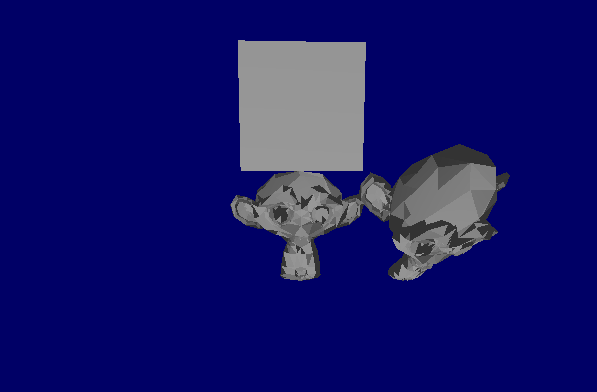
\includegraphics[scale=0.47]{images/rendu_sans_shader.png}
        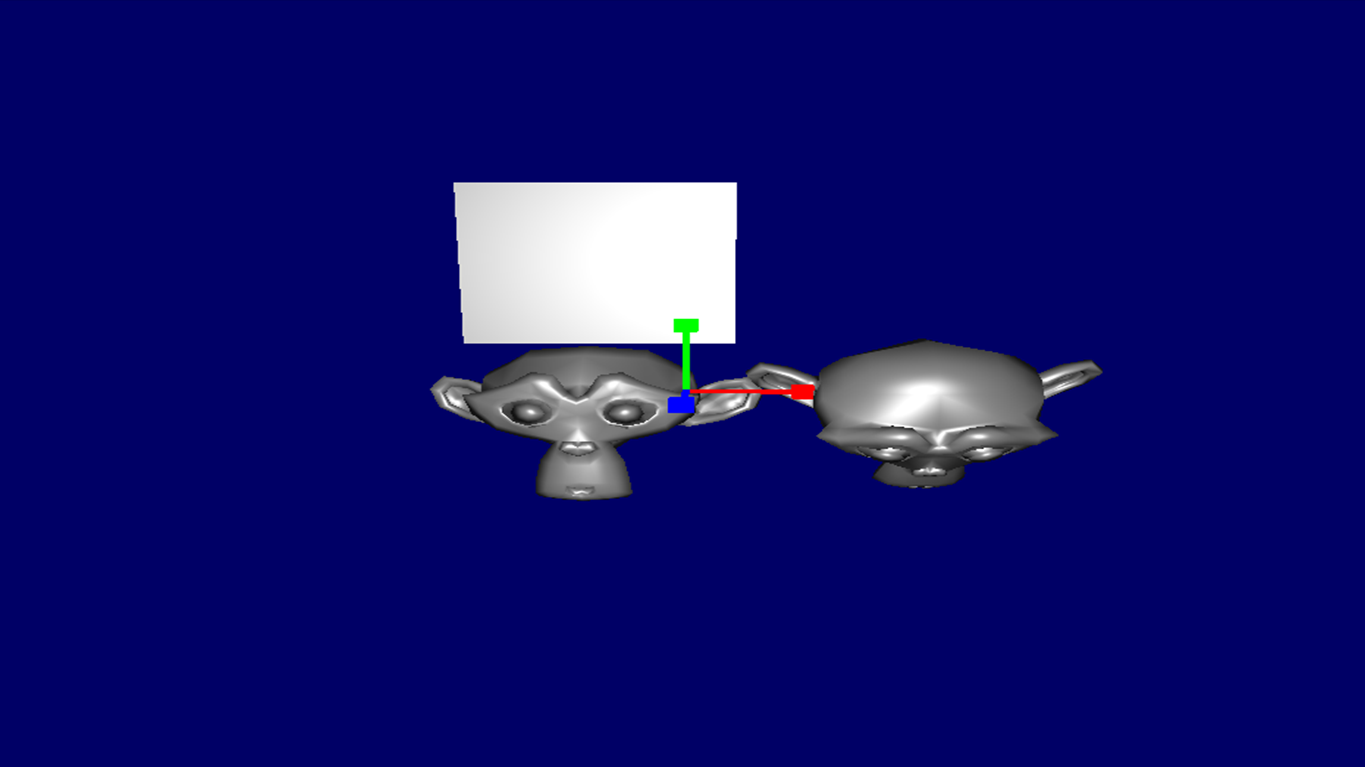
\includegraphics[scale=0.3]{images/singe_shaders.png}
	\caption{\label{fig:screenRenduSansShader.png} Comparaison de rendu avec et sans shaders \protect}
\end{figure}

\subsubsection{La spécularité}
Pour améliorer le rendu, il a été choisi de rajouter une spécularité à l'aide du shader. Cet effet permet de simuler les réflections de lumière sur l'objet, comme le montre la figure \ref{fig:screenSpecular.png}.


\begin{figure}[h!]
	\centering
	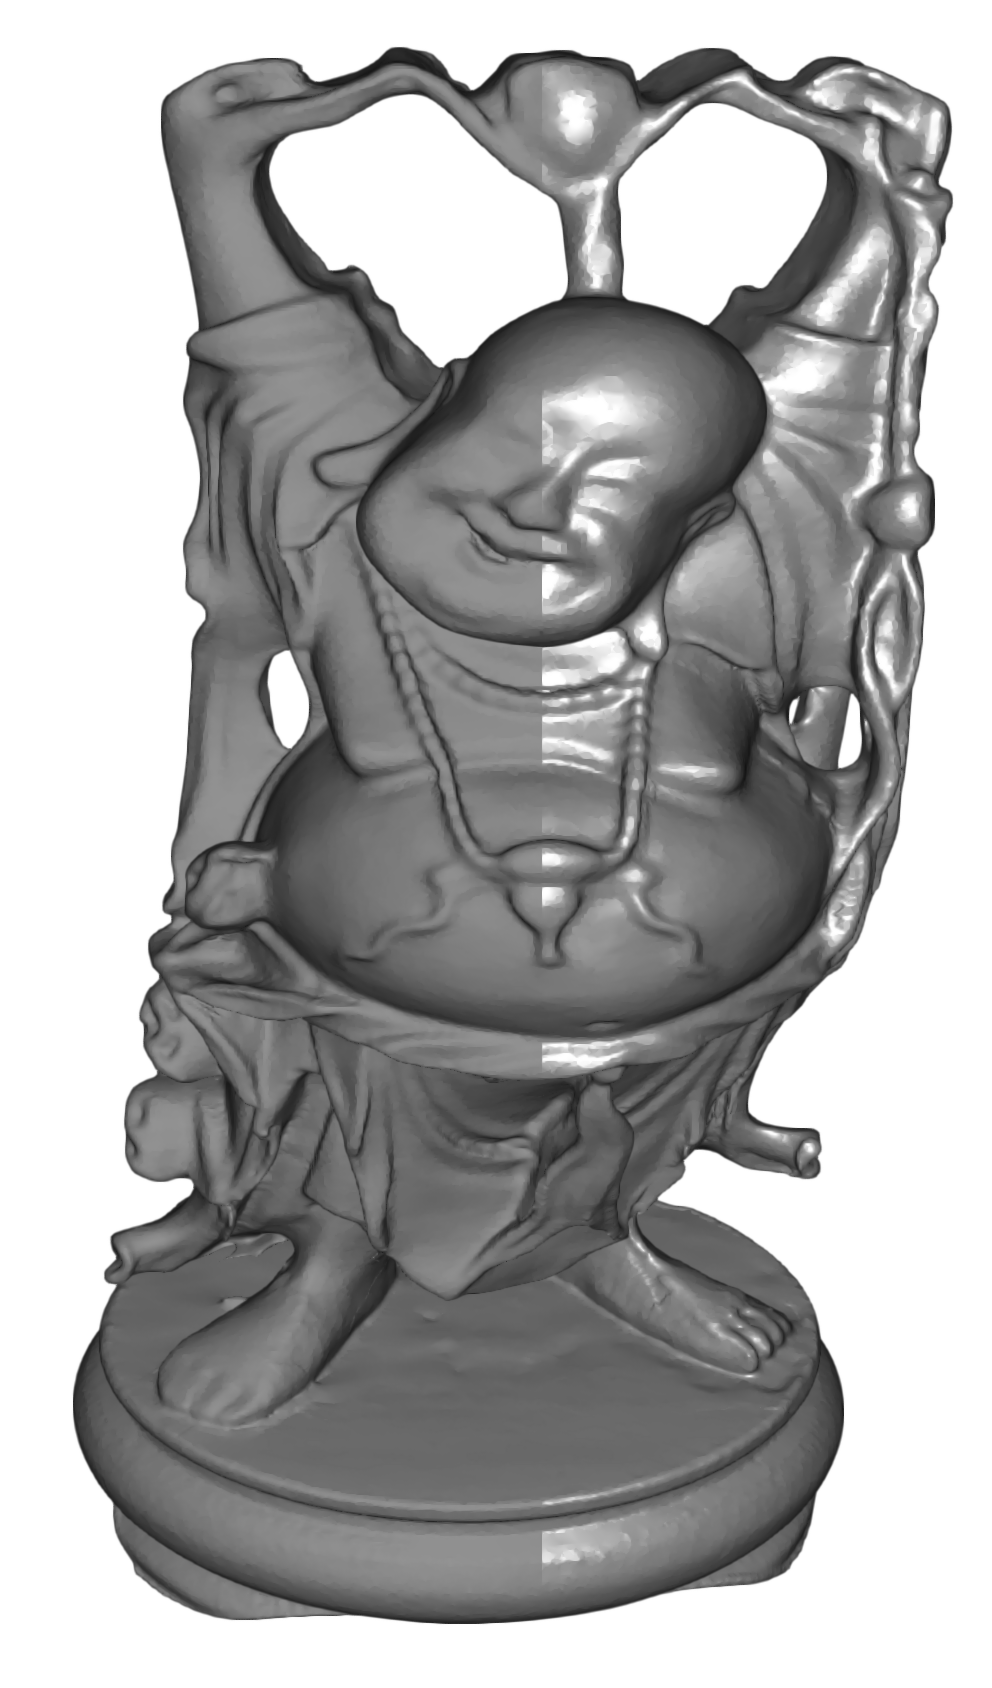
\includegraphics[scale=0.23]{images/rendu_specular.png}
	\caption{\label{fig:screenSpecular.png} Rendu avec l'ombrage de base à gauche et avec la spécularité à droite. \protect}
\end{figure}

\subsubsection{L'anti-aliasing}
Les rendus réalisés avec OpenGL présentent l'inconvénient d'avoir les bords des objets très coupants. Pour remédier à ce problème et adoucir les bords, de l'anti-aliasing est appliqué sur toute l'image (figure \ref{fig:antialiasing.png}). L'algorithme commence par trouver tous les bords contenus dans l'image et ensuite les pixels sont floutés le long du bord.
L'utilisateur a la possibilité de choisir le niveau d'itération, c'est à dire le nombre de fois que va être appliqué l'algorithme sur l'image.

\begin{figure}[h!]
	\centering
	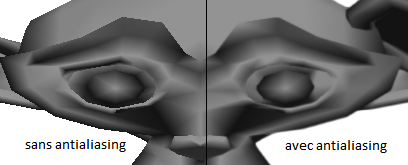
\includegraphics[scale=0.7]{images/antialiasing.png}
	\caption{\label{fig:antialiasing.png} Rendu de base à gauche et avec anti-aliasing à droite. \protect}
\end{figure}

